\documentclass{scrartcl}
\usepackage[utf8]{inputenc}
\usepackage{listings}
\usepackage{geometry}
\usepackage[T1]{fontenc}
\usepackage{appendix}
\usepackage{graphicx}
\usepackage{amsthm}
\usepackage{amssymb}
\usepackage{amsmath}
\usepackage{mathtools}
\usepackage{float}
\usepackage[UKenglish]{babel}
\usepackage{url}
\usepackage{titling}
\usepackage{multirow}
\usepackage{subcaption}

\usepackage{algorithm}
\usepackage[noend]{algpseudocode}
\usepackage{amsfonts}

\DeclarePairedDelimiter\ceil{\lceil}{\rceil}
\DeclarePairedDelimiter\floor{\lfloor}{\rfloor}
\DeclareMathOperator{\Tr}{Tr}
\DeclareMathOperator*{\argmin}{\arg\!\min}
\DeclareMathOperator*{\argmax}{\arg\!\max}

\title{Computational Statistics\\Project Report}
%\author{...}

\begin{document}

    \maketitle


    \section{Introduction}
    ...

    In diesem Projekt reimplementiere ich den vorgeschlagenen Markov Chain Monte Carlo (MCMC) Algorithmus aus dem Paper
    \cite{lau2019} und versuche die Ergebnisse der Experimente zu reproduzieren. Der hier betrachtete Paper baut auf den Ideen von
    \cite{metropolis1953,geyer1992,liu2000} und \cite{yang2019} auf.
    Der source code unter MIT Lizenz zu diesem Projekt findet sich in dem GitHub repository
    \begin{align*}
        \texttt{github.com/rinkwitz/Adaptive\_Plateau\_MCMC}\,.
    \end{align*}
    Da die Simulation der Markov chains sehr zeitaufwendig ist, kann man schon berechnete Läufe unter dem Link
    \begin{align*}
        \texttt{drive.google.com/file/d/1MHFLckoims5PYrMWPh2xkQWR0kefofgy/view?usp=sharing}
    \end{align*}
    herunterladen.

    \section{Adaptive Component-wise Multiple-Try Metropolis Algorithm} Der Kernalgorithmus
    des Papers \cite{lau2019} besteht aus einem MCMC Algorithmus der drei Eigenschaften erfüllt. Der Algorithmus schlägt
    beim sampling mehrere Vorschläge aus verschiedenen Plateauverteilungen vor. Dies passiert unabhängig für alle
    Komponenten eines samples. Die Plateauverteilungen adaptieren ihre Form in Abhängigkeit von der Frequenz der akzeptierten sample Vorschläge.

	\subsection{Plateau Proposal Distributions}
    Der MCMC Algorithmus in \cite{lau2019} verwendet zum sampling von Vorschlägen \textit{non-overlapping plateau proposal distributions}.
	Die dabei verwendete grundlegende probability distribution function $f$ ist eine Kombination einer uniform distribution
	mit exponentiell decaying tails. Dabei ist die Verteilung $f$ konstant um einen Mittelwert $\mu$ in dem abgeschlossenen Intervall $[\mu-\delta,\mu+\delta]$ mit $\delta > 0$.
	Ausserhalb dieses Intervall folgt die Verteilung einem exponentiellen Verfall dessen tail Breite durch ein seitenabhängiges $\sigma_i >0$ bestimmt wird,
	je nachdem ob man sich auf der linken oder rechten Seite des Intervalls $[\mu-\delta,\mu+\delta]$ befindet. Definiert man
	eine unnormalisierte Verteilungsfunktion
	\begin{align*}
		\tilde{f}(y;\mu,\delta,\sigma_1,\sigma_2)&=\begin{cases}
			\exp\left( -\frac{1}{2\sigma_1^2}[y-(\mu-\delta)]^2 \right)&\quad ,y<\mu-\delta\\
           1&\quad ,\mu-\delta\leq y\leq\mu+\delta\\
           \exp\left( -\frac{1}{2\sigma_2^2}[y-(\mu+\delta)]^2 \right)&\quad ,y>\mu+\delta
		\end{cases}
	\end{align*}
    und berechnet das folgende Integral
    \begin{align*}
        C(\delta,\sigma_1,\sigma_2)&=\int\limits_{-\infty}^\infty\tilde{f}(y;\mu,\delta,\sigma_1,\sigma_2) dy\\
        &= \int\limits_{-\infty}^{\mu-\delta}\exp\left( -\frac{1}{2\sigma_1^2}[y-(\mu-\delta)]^2 \right)dy+
        \int\limits_{\mu-\delta}^{\mu+\delta}1dy+
        \int\limits_{\mu+\delta}^{\infty}\exp\left( -\frac{1}{2\sigma_2^2}[y-(\mu+\delta)]^2 \right)dy\\
        &=\frac{\sqrt{2\pi\sigma_1^2}}{2}+2\delta+\frac{\sqrt{2\pi\sigma_1^2}}{2}
    \end{align*}
    als die Summen von 2 halben Gausschen Integralen und einem Integral über eine konstatne Funktion, dann ergibt sich die normalisierte Verteilungsfunktion $f(y;\mu,\delta,\sigma_1,\sigma_2)=C(\delta,\sigma_1,\sigma_2)^{-1}\tilde{f}(y;\mu,\delta,\sigma_1,\sigma_2)$ \cite{lau2019}.
    Mithilfe von $f$ kann man die Plateau probability density distributions $T_{j,k}$, $j\in\{1,\dots,M\}$ für die trial proposals der $k$-ten Komponente definieren als
    \begin{align*}
        T_{j,k}(x,y)&=\begin{cases}
                          f(y;x,\delta_1,\sigma,\sigma)&,j=1\\
                          \frac 12 f(y;x-(2j-3)\delta-\delta_1,\delta,\sigma,\sigma)+\frac 12 f(y;x+(2j-3)\delta+\delta_1,\delta,\sigma,\sigma)&,j=2,\dots M-1\\
                          \frac 12 f(y;x-(2M-3)\delta-\delta_1,\delta,\sigma_0,\sigma)+\frac 12 f(y;x+(2M-3)\delta+\delta_1,\delta,\sigma,\sigma_1)&,j=M
        \end{cases}
    \end{align*}
    mit Werten $\delta_1,\delta,\sigma,\sigma_0,\sigma_1>0$. In Figure \ref{trial_proposals}
    sieht man die trial proposal propability density distributions für die Parameter $M=5, \delta_1=\delta=1,\sigma=0.05,\sigma_0=\sigma_1=0.5$. Man erkennt, dass sich die
    Verteilungen nur an ihren exponential decaying tails überschneiden. Die äußeren tails fallen durch die größeren $\sigma_0, \sigma_1$ Werte
    flacher ab als die restlichen tails. In dem Paper \cite{lau2019} verwenden die Autoren durchgehend die Werte $\delta=\delta_1=2,\sigma=0.05,\sigma_0=\sigma_1=3$.

    \begin{figure}
        \centering
        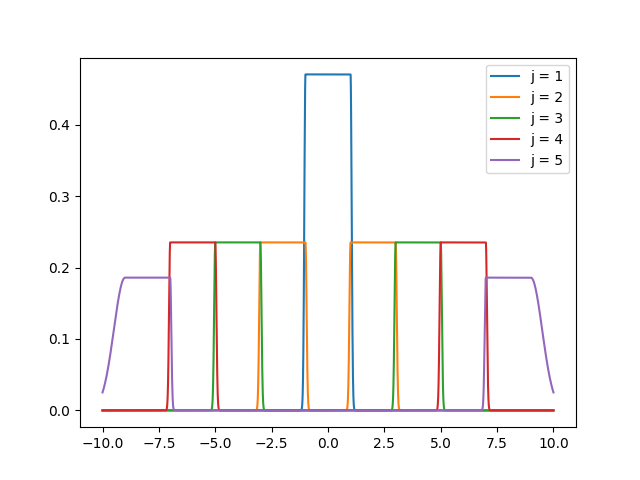
\includegraphics[scale=0.6]{../figs/fig_2b.png}
        \caption{Trial proposal propability density distributions for $M=5$}
        \label{trial_proposals}
    \end{figure}

    \subsection{Component-wise Multiple-Try Metropolis} Der \textit{Component-wise Multiple-Try Metropolis} Algorithmus \cite[Algorithm 1]{lau2019},
    welcher die Grundlage des Sampling Verfahrens bildet, startet von einer Startposition
	$x_0\in\mathbb{R}^d$. Für jede MCMC Realisationen $x_n$ mit $n\in\{1,\dots,N\}$ wird für jede der $d$ Komponenten das folgende Verfahren
	angewendet. Sei $x=(x_1,\dots,x_d)$ der letzte gesampelte Kandidat des MCMC Algorithmus, dann schlägt der Algorithmus trials $z_j$
    für $i=1,\dots,M$ in dem er diese aus den Verteilungen $T_{j,k}(x_k,\cdot)$ sampelt. In meiner Reeimplementierung des Papers verwende
    ich dazu ein rejection sampling Verfahren \cite{rejection_sampling}. Dabei verwende ich eine gleichförmige Verteilung zum Erzeugen der samples über den folgenden Intervallen
%    \begin{itemize}
%        \item $j=1:I_1=[x_k-\delta_1-t_1,x_k+\delta_1+t_1]$ mit $t_1 = \sqrt{-2\sigma^2\log(0.0001C(\delta_1,\sigma,\sigma))}$,
%        \item $j=2,\dots,M-1:I_2=[x_k-2(j+1)\delta-\delta_1-t_2,x-2j\delta-\delta_1+t_2]\cup[x_k+2j\delta+\delta_1-t_2,x+2(j+1)\delta-\delta_1+t_2]$ mit $t_2=\sqrt{-2\sigma^2\log(0.0002C(\delta,\sigma,\sigma))}$, und
%        \item $j=M:I_3=[x_k-2(M+1)\delta-\delta_1-t_{32},x_k-2M\delta-\delta_1+t_{31}]\cup[x_k+2M\delta+\delta_1-t_{31},x_k+2(M+1)\delta+\delta_1+t_{32}]$ mit $t_{31}=\sqrt{-2\sigma^2\log(0.0002C(\delta,\sigma,\sigma_0))},t_{32}=\sqrt{-2\sigma_0^2\log(0.0002C(\delta,\sigma,\sigma_0))}$.
%    \end{itemize}
    \begin{align*}
        I_j = \begin{cases}
                  [x_k-\delta_1-t_1,x_k+\delta_1+t_1]\\\text{ for }j=1\text{ with }t_1 = \sqrt{-2\sigma^2\log(0.0001C(\delta_1,\sigma,\sigma))},\vspace{.25cm}\\
                  [x_k-2(j+1)\delta-\delta_1-t_2,x-2j\delta-\delta_1+t_2]\cup[x_k+2j\delta+\delta_1-t_2,x+2(j+1)\delta-\delta_1+t_2]\\\text{ for }j=2,\dots,M-1\text{ with }t_2=\sqrt{-2\sigma^2\log(0.0002C(\delta,\sigma,\sigma))},\text{ or}\vspace{.25cm}\\
                  [x_k-2(M+1)\delta-\delta_1-t_{32},x_k-2M\delta-\delta_1+t_{31}]\cup[x_k+2M\delta+\delta_1-t_{31},x_k+2(M+1)\delta+\delta_1+t_{32}]\\\text{ for }j=M\text{ with }t_{31}=\sqrt{-2\sigma^2\log(0.0002C(\delta,\sigma,\sigma_0))},t_{32}=\sqrt{-2\sigma_0^2\log(0.0002C(\delta,\sigma,\sigma_0))}.
        \end{cases}
    \end{align*}
    Diese Intervalle ermöglichen es in dem Bereich aus $T_{j,k}(x_k,\cdot)$ effektiv zu samplen wo die probability density function größer als $0.0001$ ist.
    Dazu sampelt man solange ein $u\sim U(0,1)$ und ein $y\sim U(I_i)$ bis
    \begin{align*}
        u < \frac{T_{j,k}(x_k,y)}{c|I_i|}
    \end{align*}
    erfüllt ist wobei $|I_j|$ die Breite des verwendeten Intervalls $I_j$ ist, $g_j$ die probability density function der gleichmäßigen Verteilung über $I_j$ ist und $c_j$ situationsabhängig folgende Werte hat
    \begin{itemize}
        \item $j=1:\quad c_1=\sup\limits_{y\in I_1}\frac{T_{1,k}(x_k,y)}{g_1(y)}=\frac{|I_1|}{C(\delta_1,\sigma,\sigma)}$,
        \item $j=2:\quad c_j=\sup\limits_{y\in I_j}\frac{T_{j,k}(x_k,y)}{g_j(y)}=\frac{|I_j|}{2C(\delta,\sigma,\sigma)}$, und
        \item $j=M:\quad c_M=\sup\limits_{y\in I_M}\frac{T_{M,k}(x_k,y)}{g_M(y)}=\frac{|I_M|}{2C(\delta,\sigma,\sigma_0)}$.
    \end{itemize}
    Danach werden die zu den trials assoziierten weights
    \begin{align*}
        w_{j,k}&=\pi((z_j;x_{[-k]}))T_{j,k}(x_k,z_j)\lambda_{j,k}(x_k,z_j),\quad\text{for }j=1,\dots,M
    \end{align*}
    berechnet wobei $(z;x_{[-i]})\in\mathbb{R}^d$ den Vektor bezeichnet, der in allen Einträgen bis auf den $i$-ten mit $x$ identisch ist. Der $i$-te Eintrag nimmt hierbei den Wert $z$ an.
    Zudem wird die nicht-negative und symmetrische Funktion
    \begin{align*}
        \lambda_{j,k}(x,y)&=|y-x|^{2.5}%T_{j,k}(x,y)
    \end{align*}
    verwendet. Dabei beziehen sich die Autoren von \cite{lau2019} auf die Ergebnisse von \cite{yang2019}. Ein hohes Gewicht bekommen somit Vorschläge $(z_j;x_{[-k]})$, die eine hohe Wahrscheinlichkeit bezüglichd der
    Zielverteilung $\pi$ haben, deren neuer Vorschlag $z_j$ für die $k$-te Komponente bezüglich $T_{j,k}(x_k,\cdot)$ eine hohe Wahrscheinlichkeit
    und wegen der potenzierten Abstandsfunktion $\lambda_{j,k}$ weit genug von $x_k$ entfernt ist.
    Proportional zu den Gewichten $w_{1,k},\dots,w_{M,k}$ wird dann ein $y\in\{z_1,\dots,z_M\}$ zufällig gezogen und für $j=1,\dots,M-1$ sampelt der Algorithmus
    $x_j^*\sim T_{j,k}(y,\cdot)$. Schließlich berechnet man
    \begin{align*}
        \alpha&=\min\left\{ 1,\frac{w_{1,k}(z_1,x)+\dots+w_{M,k}(z_M,x)}{w_{1,k}(x_1^*,(y;x_{[-k]}))+\dots+w_{M-1,k}(x_{M-1}^*,(y;x_{[-k]}))+w_{M,k}(x_k,(y;x_{[-k]}))} \right\}
    \end{align*}
    und nimmt mit dieser Wahrscheinlichkeit $\alpha$ den neuen Vorschlag an und setzt $x_n=(y;x_{[-k]})$. Andernfalls verbleibt der Algorithmus
    bei dem alten Vorschlag und setzt $x_n=x$.

    \subsection{Adaption of Proposal Distributions}
    In \cite{lau2019} wird vorgeschlagen die Breiten $\delta$ und $\delta_0$ der Plateauverteilungen adaptiv anzupassen.
    In meiner Implementierung wird alle $L$ Iterationen gemessen, wie groß die Anzahlen der ausgewählten Vorschläge $c_{j,k}$ von den Plateauverteilungen $T_{j,k}$ in diesem Intervall sind.
    Wird die mittlere Plateauverteilung überdurschnittlich oft aufgerufen, also $c_{j,k}>L\eta_1$ mit $\eta_1\in(0,1)$, dann
    geht der Algorithmus davon aus, dass die Plateaus zu breit sind und halbiert dementsprechend $\delta$ und $\delta_1$ für
    die folgenden Iterationen. Werden hingegen die äußersten Plateauverteilungen überdurchschnittlich oft ausgewählt, also
    $c_{M,k}>\eta_2L$ mit $\eta_2\in(0,1)$, dann geht der Algorithmus davon aus, dass die Plateaus zu klein sind und verdoppelt
    somit $\delta$ und $\delta_1$. Die Adaptionen finden nur mit einer immer kleiner werdenden Wahrscheinlichkeit von $\max(0.99^{n-1},1/\sqrt{n})$ statt. Diese Implementierung der Adaptionsvorgehensweise basiert auf \cite[Algorithm 2]{lau2019}.

    \section{Experiments and Results}

    \subsection{Performance Measures}
    \subsubsection{Integrated Autocorrelation Times}
    Die Autoren in dem Paper \cite{lau2019} verwenden zwei performance measures, um die Wirksamkeit des implementierten
    Algorithmus zu untersuchen. Dies ist zum einen die integrated autocorrelation times (ACT), welche in $R$ MCMC
    Simulationen mit jeweils $N$ Schritten für $K$ Komponenten berechnet wird. Sei im Folgenden
    $X_t^{(r)}=(X_{t,1}^{(r)},\dots,X_{t,K}^{(r)})$ das Ergebnis der $r$-ten MCMC Simulation bei Schritt $t$, wobei
    $r\in\{1,\dots,R\}$ und $t\in\{1,\dots,N\}$. Die Implementierung benutzt einen \textit{initial positive sequence estimator}
    wie ihn \cite{geyer1992} verwendet. Dafür wird zunächst die komponentenweise die empirische Autokovarianz bestimmt um
    die lagged autocovariance $\gamma_{i,k}^{(r)}$ mit $k\in\{1,\dots,K\}$ zu schätzen. Dabei ist
    \begin{align*}
        \hat{\gamma}_{t,k}^{(r)}&=\frac{1}{N}\sum\limits_{i=1}^{N-t}(X_{i,k}^{(r)}-\bar{X_k}^{(r)})(X_{i+t,k}^{(r)}-\bar{X_k}^{(r)})
    \end{align*}
    wobei $\bar{X_k}^{(r)}=1/N\sum\nolimits_{i=1}^NX_{i,k}^{(r)}$ das arithmetische Mittel $k$-ten Komponente in der $r$-ten
    Simulation bezeichnet. Danach schauen wir uns die Summen
    \begin{align*}
        \hat{\Gamma}_{m,k}^{(r)} &= \hat{\gamma}_{2m,k}^{(r)} + \hat{\gamma}_{2m+1,k}^{(r)}
    \end{align*}
    von benachbarten Autokovarianzen Paaren an. Schließlich ergibt sich die integrated autocorrelation times als
    \begin{align*}
        \text{ACT}_k^{(r)}&=-\hat{\gamma}_{0,k}^{(r)}+2\sum\limits_{i=0}^{m}\hat{\Gamma}_{m,k}^{(r)}
    \end{align*}
    wobei $m$ die größte natürliche Zahl ist, sodass $\hat{\Gamma}_{i,k}^{(r)} > 0$ für alle $i\in\{1,\dots,m\}$ gilt
    \cite{geyer1992}. Schränkt man dies noch weiter ein und fordert zusätzlich noch, dass
    die Teilfolge $(\hat{\Gamma}_{i,k}^{(r)})_{i=1,\dots,m}$ monoton sein muss, so erhält man einen
    \textit{initial monotone sequence estimator} \cite{geyer1992}. Dabei zeigt eine kleinere autocorrelation times an, dass
    aufeinanderfolgende samples eine kleinere Korrelation haben \cite{lau2019}.
    \subsubsection{Average Squared Jump Distance}
    Ein weiteres Performance Maß ist die average squared jump distance (ASJD)
    \begin{align*}
        \text{ASDJ}_k^{(r)}=\frac{1}{N}\sum\limits_{i=1}^N|X_{i,k}^{(r)}-X_{i-1,k}^{(r)}|^2
    \end{align*}
    für die $k$-te Komponente und die $r$-te Wiederholung der Markov chain \cite{lau2019}.
    Hierbei sind größere ASJD Werte zu bevorzugen, da sie anzeigen, dass der state-space besser erkundet wird \cite{lau2019}.

    \subsection{Experiments}
    \subsubsection{Target Distributions}
    Als Experimente um die Performance der adaptiven plateau-basierten MCMC Methode zu testen, wird in \cite{lau2019} versucht vier Zelverteilungen
    mit der Markov chain zu approximieren. Die Zielverteilungen sind dabei
    \begin{itemize}
        \item $\pi_1:$ a mixture of 4-dimensional Gaussians $\frac12\mathcal{N}(\mu_1,\Sigma_1)+\frac12\mathcal{N}(\mu_2,\Sigma_2)$ with $\mu_1=(5,5,0,0)^T,\mu_2=(15,15,0,0)^T,\Sigma_1=\text{diag}(6.25,6.25,6.25,0.01),\Sigma_2=\text{diag}(6.25,6.25,0.25,0.01)$,
        \item $\pi_2:$ an 8-dimensional banana distribution with density $f\circ\phi$, wobei $f$ die Dichte einer 8-dimensionalen Normalverteilung $\mathcal{N}(0,\Sigma_3)$ mit $\Sigma_3=\text{diag}(100,1,\dots,1)$ und $\phi(x)=(x_1,x_2+0.03x_1^2-3,x_3,\dots,x_8)$ für $x\in\mathbb{R}^8$ ist,
        \item $\pi_3:$ a perturbed 2-dimensional Gaussian mit unnormalisierter Wahrscheinlichkeitsdichte $\tilde{\pi_3}(x)=\exp\left( -x^TAx-\cos\left( \frac{x_1}{0.1} \right) -0.5\cos\left( \frac{x_2}{0.1} \right) \right)$ für $x\in\mathbb{R}^2$ mit
        $A=\begin{pmatrix}
                    1 & 1\\
                    1 & 3/2
        \end{pmatrix}$, und
        \item $\pi_4:$ eine 1-dimensional bi-stable Verteilung mit unnormalisierter Verteilung $\tilde{\pi_4}(x)=\exp\left( -x^4+5x^2-\cos\left( \frac{x}{0.02} \right) \right)$ für $x\in\mathbb{R}$.
    \end{itemize}
    Diese Verteilungen sind in Figure \ref{target_distributions} dargestellt, welche sich an \cite[Figure 3]{lau2019} orientiert. Die Darstellung
    von $\pi_2$ in Figure \ref{target_distributions_pi_2} resultiert aus einer dimensionsreduzierte Vereinfachung, da ein Marginal mit 6 Integrationsvariablen zu
    rechenintensiv gewesen ist. Dies erkennt man auch daran, dass die Wahrscheinlichkeitsdichte hier größer ist als diejenige in \cite{lau2019}.
    \begin{figure}
        \centering
        \begin{subfigure}{.45\textwidth}
              \centering
              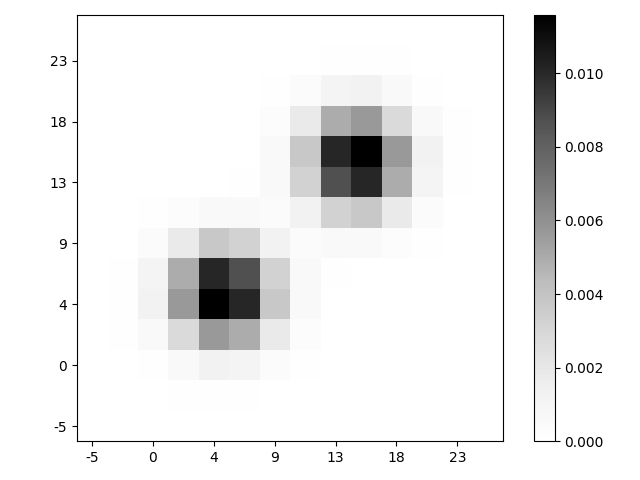
\includegraphics[width=.8\linewidth]{../figs/fig_3_pi_1.png}
              \caption{Joint PDF of components 1 and 2 of $\pi_1$}
              \label{target_distributions_pi_1}
        \end{subfigure}
        \begin{subfigure}{.45\textwidth}
              \centering
              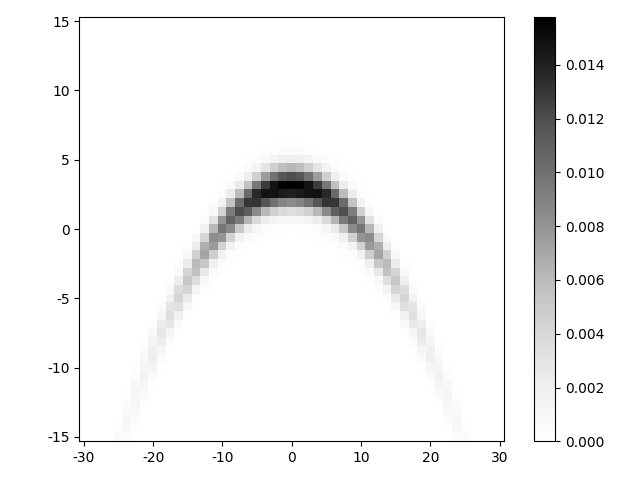
\includegraphics[width=.8\linewidth]{../figs/fig_3_pi_2.png}
              \caption{Joint PDF of components 1 and 2 of $\pi_2$}
              \label{target_distributions_pi_2}
        \end{subfigure}
        \begin{subfigure}{.45\textwidth}
              \centering
              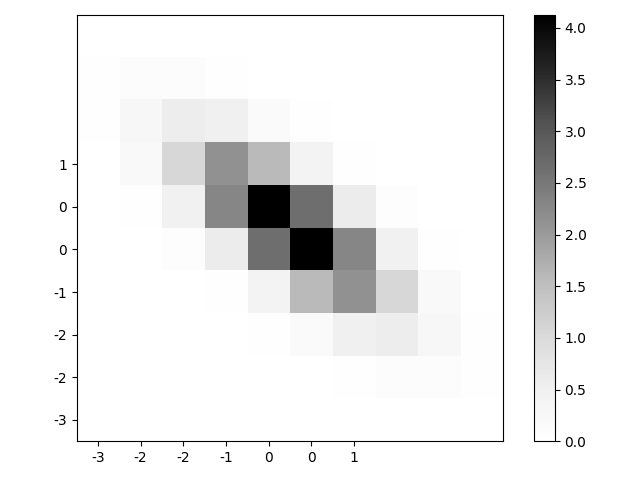
\includegraphics[width=.8\linewidth]{../figs/fig_3_pi_3.png}
              \caption{PDF of $\pi_3$}
              \label{target_distributions_pi_3}
        \end{subfigure}
        \begin{subfigure}{.45\textwidth}
              \centering
              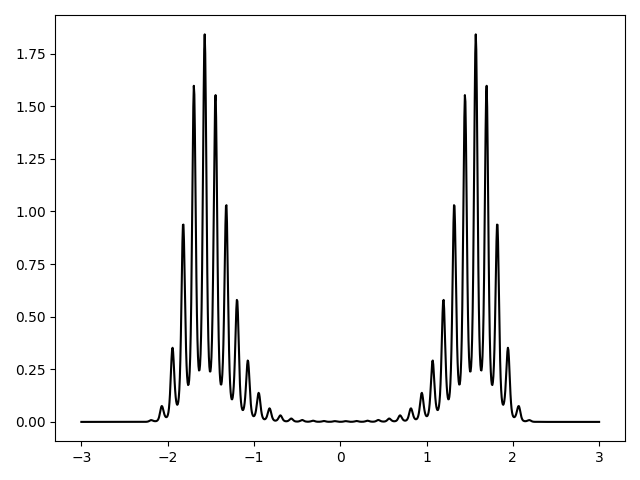
\includegraphics[width=.8\linewidth]{../figs/fig_3_pi_4.png}
              \caption{PDF of $\pi_4$}
              \label{target_distributions_pi_4}
        \end{subfigure}
        \caption{Overview of target distributions}
        \label{target_distributions}
    \end{figure}

    \subsubsection{Simulation Parameter Settings}
    Für die 4 Zielverteilungen werden je $R=200$ MCMC Simulaitionen durchgeführt mit $N=4000$ Iterationen für $\pi_1$, $N=10000$ Iterationen für $\pi_2$, und $N=3000$ Iterationen für $\pi_3$ und $\pi_4$.
    Die restlichen Parameter sind einheitlich für alle Simulationen. Dies sind
    \begin{itemize}
        \item $M=5$ verschiedene Plateauvorschlagsverteilungen,
        \item $\delta=\delta_1=2$ Breite der Plateaus,
        \item $\sigma=0.05$ und $\sigma_0=\sigma_1=3$ Flachheit der Plateau tails,
        \item $\eta_1=\eta_2=0.4$ mindest Anteil für eine Adaption,
        \item $L=40$ Länge des Intervalls zwischen den Adaptionen, und
        \item einen burn-in Anteil von $0.5$ aller Iterationen.
    \end{itemize}
    Diese Paramter sind bis auf $L$, für welchen es keine exakten Angaben gibt, genau wie in \cite{lau2019} gesetzt.

    \subsection{Results}
    Die zu den Experimenten zugehörigen Violinen plots findet man für die Zielverteilungen $\pi_1$, $\pi_2$, $\pi_3$ und $\pi_4$ finden sich
    in den Figures \ref{violin_plots_pi_1}, \ref{violin_plots_pi_2}, \ref{violin_plots_pi_3} und \ref{violin_plots_pi_4}. Dort findet man
    die komponenteweise Darstellung der ACT Verteilung in den Subfigures \ref{violin_plots_pi_1_act}, \ref{violin_plots_pi_2_act}, \ref{violin_plots_pi_3_act} und \ref{violin_plots_pi_1_act}, sowie
    die komponentenweise Darstellung der ASJD Verteilung in den Subfigures \ref{violin_plots_pi_1_asjd}, \ref{violin_plots_pi_2_asjd}, \ref{violin_plots_pi_3_asjd} und \ref{violin_plots_pi_4_asjd}.
    Um die Resultate besser einschätzen zu können sind in den Tabellen \ref{stat_results_act}, \ref{stat_results_log_act} und \ref{stat_results_asjd} komponentenweise der Median, mean, sowie Minimum und Maximum in gerundeter Form
    aufgeführt für ACT, log ACT und ASJD der Experimente.

    \begin{figure}[H]
        \begin{table}[H]
            \centering
            \begin{tabular}{|l|l|l|l|l|l|l|l|l|l|l|l|l|l|l|}
                \hline & $\pi_1$ & $\pi_2$ & $\pi_3$ & $\pi_4$ \\ \hline
                ...
            \end{tabular}
            \caption{Gerundete statistical results of ACT komponentenweise}
            \label{stat_results_act}
        \end{table}
    \end{figure}

    \begin{figure}[H]
        \begin{table}[H]
            \centering
            \begin{tabular}{|l|l|l|l|l|l|l|l|l|l|l|l|l|l|l|}
                \hline & $\pi_1$ & $\pi_2$ & $\pi_3$ & $\pi_4$ \\ \hline
                ...
            \end{tabular}
            \caption{Gerundete statistical results of log ACT komponentenweise}
            \label{stat_results_log_act}
        \end{table}
    \end{figure}

    \begin{figure}[H]
        \begin{table}[H]
            \centering
            \begin{tabular}{|l|l|l|l|l|l|l|l|l|l|l|l|l|l|l|}
                ...
            \end{tabular}
            \caption{Gerundete statistical results of ASJD komponentenweise}
            \label{stat_results_asjd}
        \end{table}
    \end{figure}

    \begin{figure}
        \centering
        \begin{subfigure}{0.45\textheight}
              \centering
              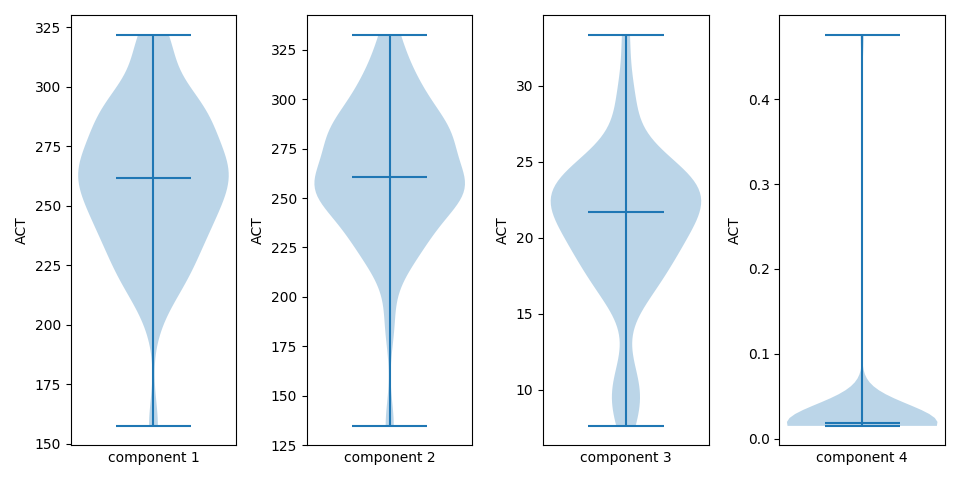
\includegraphics[width=.8\linewidth]{../figs/ACT_pi_1.png}
              \caption{komponenteweise ACT distribution für Zielverteilung $\pi_1$}
              \label{violin_plots_pi_1_act}
        \end{subfigure}
        \begin{subfigure}{0.45\textheight}
              \centering
              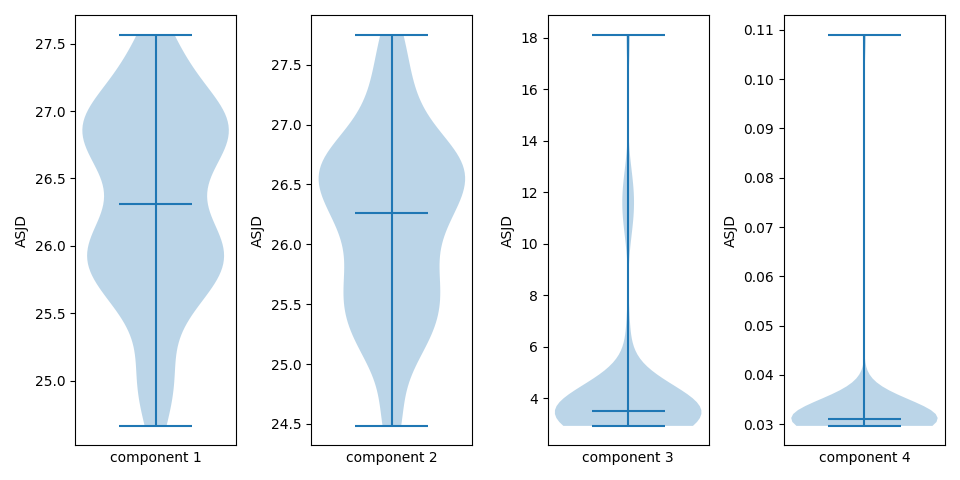
\includegraphics[width=.8\linewidth]{../figs/ASJD_pi_1.png}
              \caption{komponenteweise ASJD distribution für Zielverteilung $\pi_1$}
              \label{violin_plots_pi_1_asjd}
        \end{subfigure}
        \caption{Violin plots of performance measures for target distribution $\pi_1$}
        \label{violin_plots_pi_1}
    \end{figure}

    \begin{figure}
        \centering
        \begin{subfigure}{0.45\textheight}
              \centering
              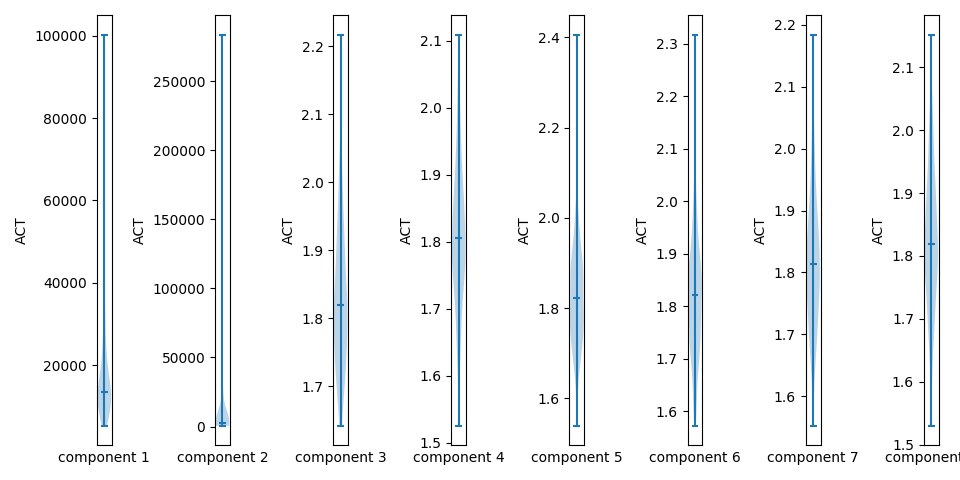
\includegraphics[width=.8\linewidth]{../figs/ACT_pi_2.png}
              \caption{komponenteweise ACT distribution für Zielverteilung $\pi_2$}
              \label{violin_plots_pi_2_act}
        \end{subfigure}
        \begin{subfigure}{0.45\textheight}
              \centering
              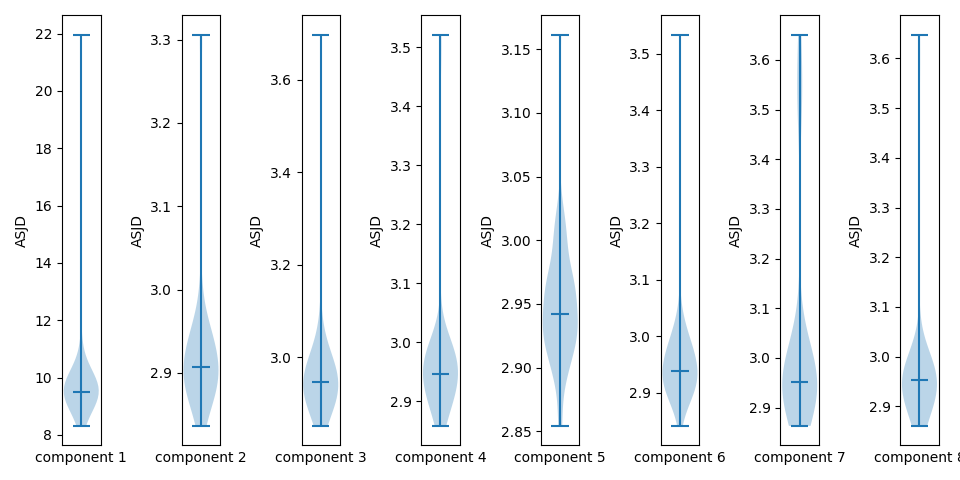
\includegraphics[width=.8\linewidth]{../figs/ASJD_pi_2.png}
              \caption{komponenteweise ASJD distribution für Zielverteilung $\pi_2$}
              \label{violin_plots_pi_2_asjd}
        \end{subfigure}
        \caption{Violin plots of performance measures for target distribution $\pi_2$}
        \label{violin_plots_pi_2}
    \end{figure}

    \begin{figure}
        \centering
        \begin{subfigure}{0.45\textheight}
              \centering
              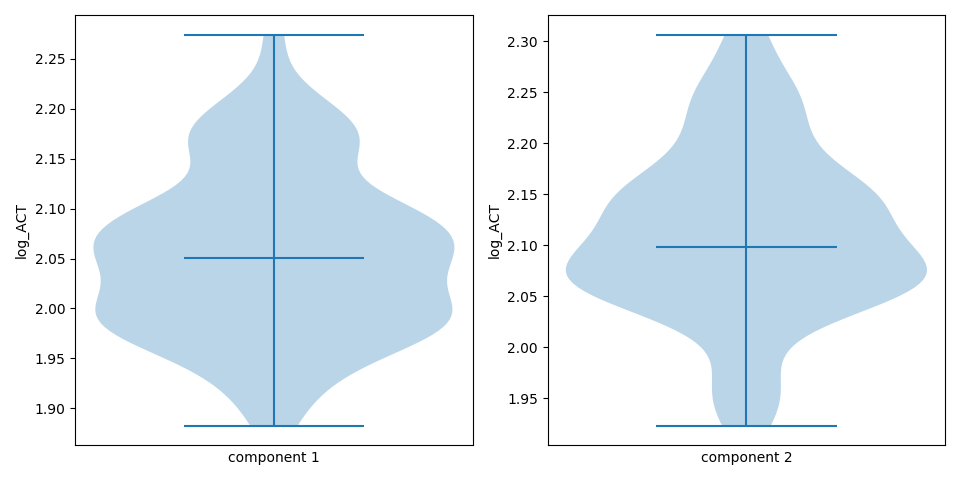
\includegraphics[width=.8\linewidth]{../figs/log_ACT_pi_3.png}
              \caption{komponenteweise log ACT distribution für Zielverteilung $\pi_3$}
              \label{violin_plots_pi_3_act}
        \end{subfigure}
        \begin{subfigure}{0.45\textheight}
              \centering
              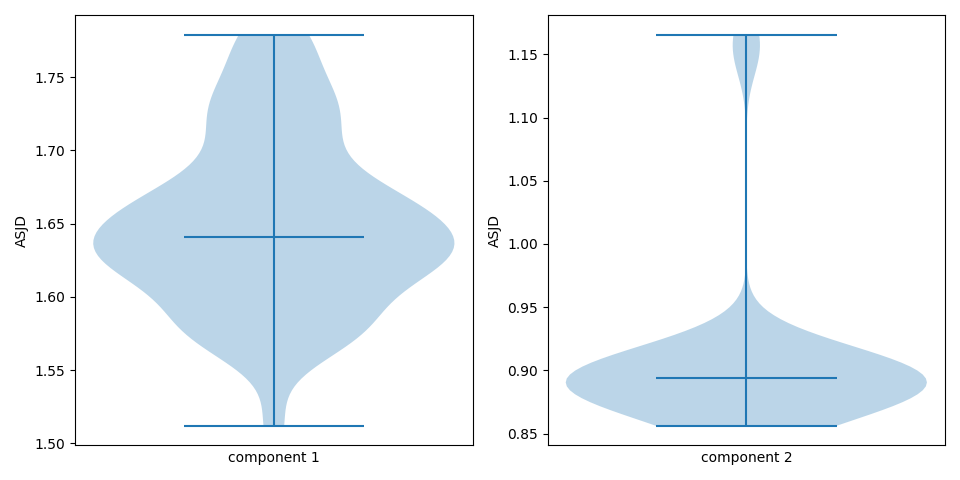
\includegraphics[width=.8\linewidth]{../figs/ASJD_pi_3.png}
              \caption{komponenteweise ASJD distribution für Zielverteilung $\pi_3$}
              \label{violin_plots_pi_3_asjd}
        \end{subfigure}
        \caption{Violin plots of performance measures for target distribution $\pi_3$}
        \label{violin_plots_pi_3}
    \end{figure}

    \begin{figure}
        \centering
        \begin{subfigure}{0.45\textheight}
              \centering
              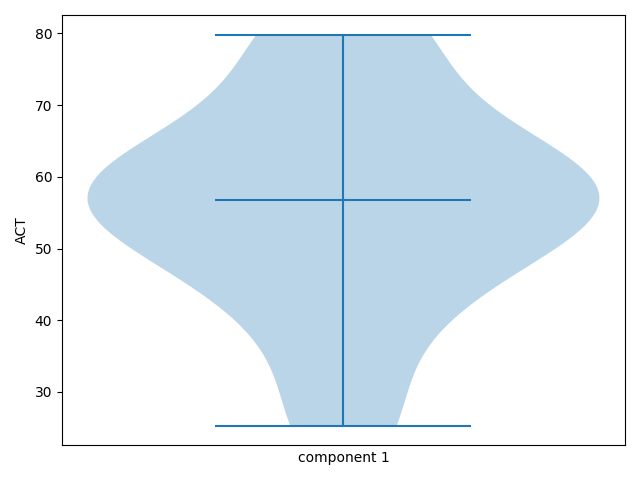
\includegraphics[width=.8\linewidth]{../figs/ACT_pi_4.png}
              \caption{komponenteweise ACT distribution für Zielverteilung $\pi_4$}
              \label{violin_plots_pi_4_act}
        \end{subfigure}
        \begin{subfigure}{0.45\textheight}
              \centering
              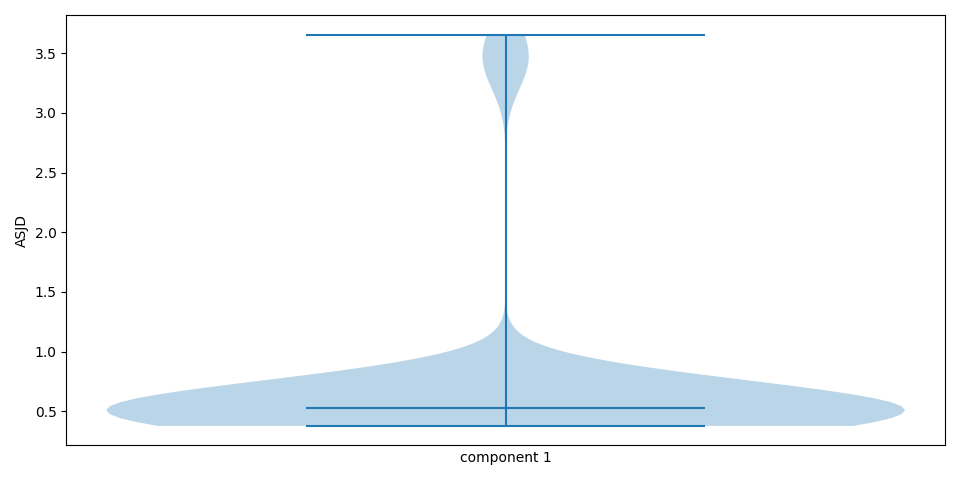
\includegraphics[width=.8\linewidth]{../figs/ASJD_pi_4.png}
              \caption{komponenteweise ASJD distribution für Zielverteilung $\pi_4$}
              \label{violin_plots_pi_4_asjd}
        \end{subfigure}
        \caption{Violin plots of performance measures for target distribution $\pi_4$}
        \label{violin_plots_pi_4}
    \end{figure}

    \section{Discussion}
    TO DO ...

    \section{Technical Details of Implementation}
    Die Reimplementierung von \cite{lau2019} ist in Python 3 geschrieben und es werden die Pakete \texttt{Numpy}, \texttt{Scipy}
    und \texttt{Matplotlib} benötigt. Die vier Simulationen zur Reproduktion der MCMC Resultate können mit des Skriptes
    \texttt{run\_simulations.py} ausgeführt werden, welches alle vier Simulationen parallelisiert mithilfe von \texttt{multiprocessing} ausführt.
    Die einstellbaren Parameter können unter \texttt{adjustable parameters} in den Skripten gefunden werden. Dabei folgen sie der Namenskonvention aus diesem Report
    und dem Paper \cite{lau2019}. Nachdem die Simulationen ausgeführt wurden, kann mit dem Skript \texttt{create\_violin\_plots.py}
    die Violinenplots für die Resultate erstellt werden. Zusätzlich gibt es noch die beiden Skripte \texttt{create\_fig\_2b.py}
    und \texttt{create\_fig\_3.py} mit denen Reproduktionen der Figures 2b und 3 aus \cite{lau2019} erstellt werden können.
    Falls man die in der Cloud schon bereitgestellten MCMC Läufe verwenden möchte, so muss man die entpackten \texttt{Numpy}-arrays in den Ordner
    \texttt{simulations} kopieren.

    \bibliographystyle{apalike}
    \bibliography{ref}
\end{document}
